\section{Bază de date filme}
În cadrul prezentei diserații a fost folosită ca bază de date pentru evaluarea experimentală baza oferita de grouplens \hyperlink{movielens}{[22]}. Aceștia pun la dispoziție mai multe seturi de date printre care:
\begin{enumerate}
	\item \textbf{MovieLens 20M Dataset}: conține 20 milioane de ratinguri oferite de 138 000 de utilizatori peste 27 000 de filme;
	\item \textbf{MovieLens 10M Dataset}: conține 10 milioane de ratinguri oferite de 72 000 de utilizatori peste 10 000 de filme;
	\item \textbf{MovieLens 1M Dataset}: conține 1 milion de ratinguri oferite de 6 000 de utilizatori peste 4 000 de filme.
\end{enumerate}

În evaluarea curentă a fost folosită cea mai recentă versiune de bază de date, actualizată la 9/2018, de dimensiune mică și anume \textit{ml-latest-small}. Această bază de date conține 100 000 de ratinguri și 3 600 de taguri aplicate peste 9 000 de filme de 600 de utilizatori. Această bază de date este un subset dintr-o bază de date cu 27 de milioane de ratinguri și 1 milion de taguri, aplicate peste 58 000 de filme de 280 000 de utilizatori.

Fiecare utilizator din \textit{ml-latest-small} a acordat ratinguri pentru cel puțin 20 de filme. Baza de date nu conține informații demografice, fiecare utilizator fiind reprezentat doar de un id.

Structura fișierelor din baza de date:
\begin{itemize}
	\item \textbf{ratings.csv}: fiecare linie din acest fișier reprezintă un rating dat de un utilizator unui film, fișierul având formatul $userId, movieId, rating, timestamp$, unde $timestamp$ reprezintă momentul de timp când a fost acordat ratingul. Fiecare rating este cuprins între 0 și 5, iar între ratinguri este unpas de 0.5;
	\item \textbf{movies.csv}: conține metadate despre filme precum titlul și genul. Formatul fișierului este următorul: $movieId, title, genres$. Titlul conține și anul de apariție a filmului sub forma \textit{Titlu (an)}. Genul poate fi unul sau mai multe dintre următoarele: \textit{Action, Adventure, Animation, Children's, Comedy, Crime, Documentary, Drama, Fantasy, Film-Noir, Horror, Musical, Mystery Romance, Sci-Fi, Thriller, War Western, (no genres listed)}.
	\item \textbf{links.csv}: conține referințele către site-urile movielens, imdb și themoviedb sub următorul format: $movieId,imdbId,tmdbId$.
	\item \textbf{tags.csv}: fiecare linie conține un tag aplicat de un utilizator unui film, fișierul având următorul format $userId,movieId,tag,timestamp$. Fiecare tag este reprezentat de un cuvânt sau de o scurtă frază.
\end{itemize}

\section{Bază de date postere}
În ceea ce privește baza de date pentru postere, aceasta a fost construită în cadrul dezvoltării prezentei lucrări cu ajutorul a două elemente: fișierul de \textit{links} din setul de date \textit{ml-latest-small} și cu API-ul pus la dispoziție de către platforma \textbf{themoviedb.org} \hyperlink{themoviedb}{[24]}.

Procesul de construcție a acestui set de postere pentru filme poate fi rezumat pe pași după cum urmează:
\begin{enumerate}
	\item \textbf{Pasul 1}: extragerea id-urilor filmelor aferente platformei themoviedb.org;
	\item \textbf{Pasul 2}: pentru fiecare film se face un request către API pentru a lua lista de postere pentru filmul curent;
	\item \textbf{Pasul 3}: având adresele posterelor pentru filmul curent, se descarcă și se salvează posterele la dimensiunea originală într-un folder specific filmului.
\end{enumerate}
Din punct de vedere al implementării putem menționa funcțiile:
\begin{lstlisting}[language=Python, caption=Construcția setul de date cu postere]
def get_tmdb_posters(tmdb_api_key, max_movie_posters=10):
    # pasul 1    
    tmdb_movies_id = get_tmdb_ids()
    # pasul 2 - 3
    download_images(tmdb_api_key, tmdb_movies_id, max_movie_posters)

# unde download_images are urmatoarea definitie:
def download_images(tmdb_api_key, tmdb_movies_id, max_movie_posters=10):
\end{lstlisting}
unde:
\begin{itemize}
	\item \textbf{tmdb\_api\_key} este api key-ul unic asociat unui cont pe platforma themoviedb.org care a solicitat acces la API-ul platformei;
	\item \textbf{max\_movie\_posters} definește care este numărul maxim de postere care va fi descărcat pentru un film. Numărul de postere descărcate poate fi mai mic în cazul în care nu sunt cel puțin max\_movie\_posters.
\end{itemize}

\begin{figure}[!tbp]
  \begin{subfigure}[b]{0.3\textwidth}
    \includegraphics[width=9cm,height=5cm,keepaspectratio]{img_4_1}
  \end{subfigure}
  \hfill
  \begin{subfigure}[b]{0.3\textwidth}
    \includegraphics[width=9cm,height=5cm,keepaspectratio]{img_4_2}
  \end{subfigure}
  \hfill
  \begin{subfigure}[b]{0.3\textwidth}
    \includegraphics[width=9cm,height=5cm,keepaspectratio]{img_4_3}
  \end{subfigure}
  \hfill
  \begin{subfigure}[b]{0.3\textwidth}
    \includegraphics[width=9cm,height=5cm,keepaspectratio]{img_4_4}
  \end{subfigure}
  \hfill
  \begin{subfigure}[b]{0.3\textwidth}
    \includegraphics[width=9cm,height=5cm,keepaspectratio]{img_4_5}
  \end{subfigure}
  \hfill
  \begin{subfigure}[b]{0.3\textwidth}
    \includegraphics[width=9cm,height=5cm,keepaspectratio]{img_4_6}
  \end{subfigure}
  \caption[Exemple de postere]{Exemplu de postere pentru filmul Paddington 2.}
\end{figure}

\section{Rezultate clusterizare postere}

\subsection{Sanity check}
Pentru testarea validității clasterelor un test de sanity check în care s-au luat opt filme și s-a încercat clasificarea lor în șapte clastere folosind caracteristicile extrase din rețelele preantrenate VGG16, VGG19, InceptionV3, ResNet50 și NASNet, clasterele create cu kNN iar evaluarea este făcută atât vizual cât și prin urmărirea evoluției metricii silhouette de la 2 la 7 clastere. Posterele de input pentru sanity check sunt prezentate în figura 4.2.
\begin{figure}[!tbp]
  \centering
  \begin{subfigure}[b]{0.48\textwidth}
    
\includegraphics[width=\textwidth]{img_4_7}
  \end{subfigure}
  \hfill
  \begin{subfigure}[b]{0.48\textwidth}
    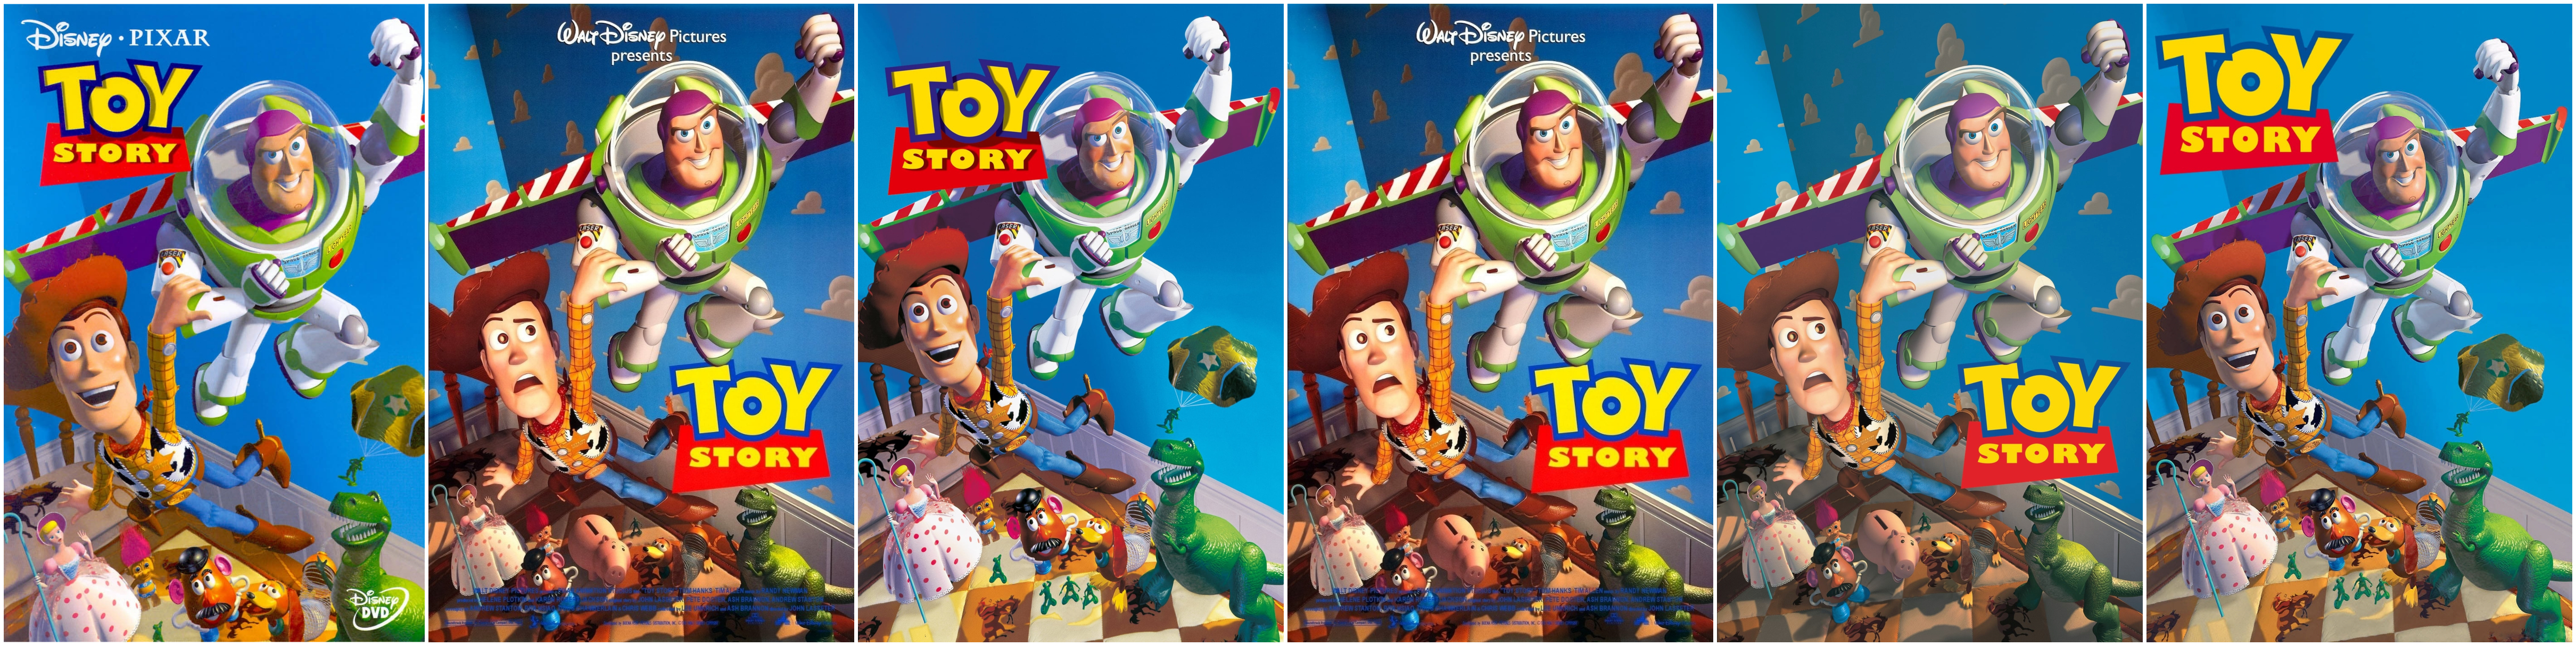
\includegraphics[width=\textwidth]{img_4_8}
  \end{subfigure}
    \hfill
  \begin{subfigure}[b]{0.48\textwidth}
    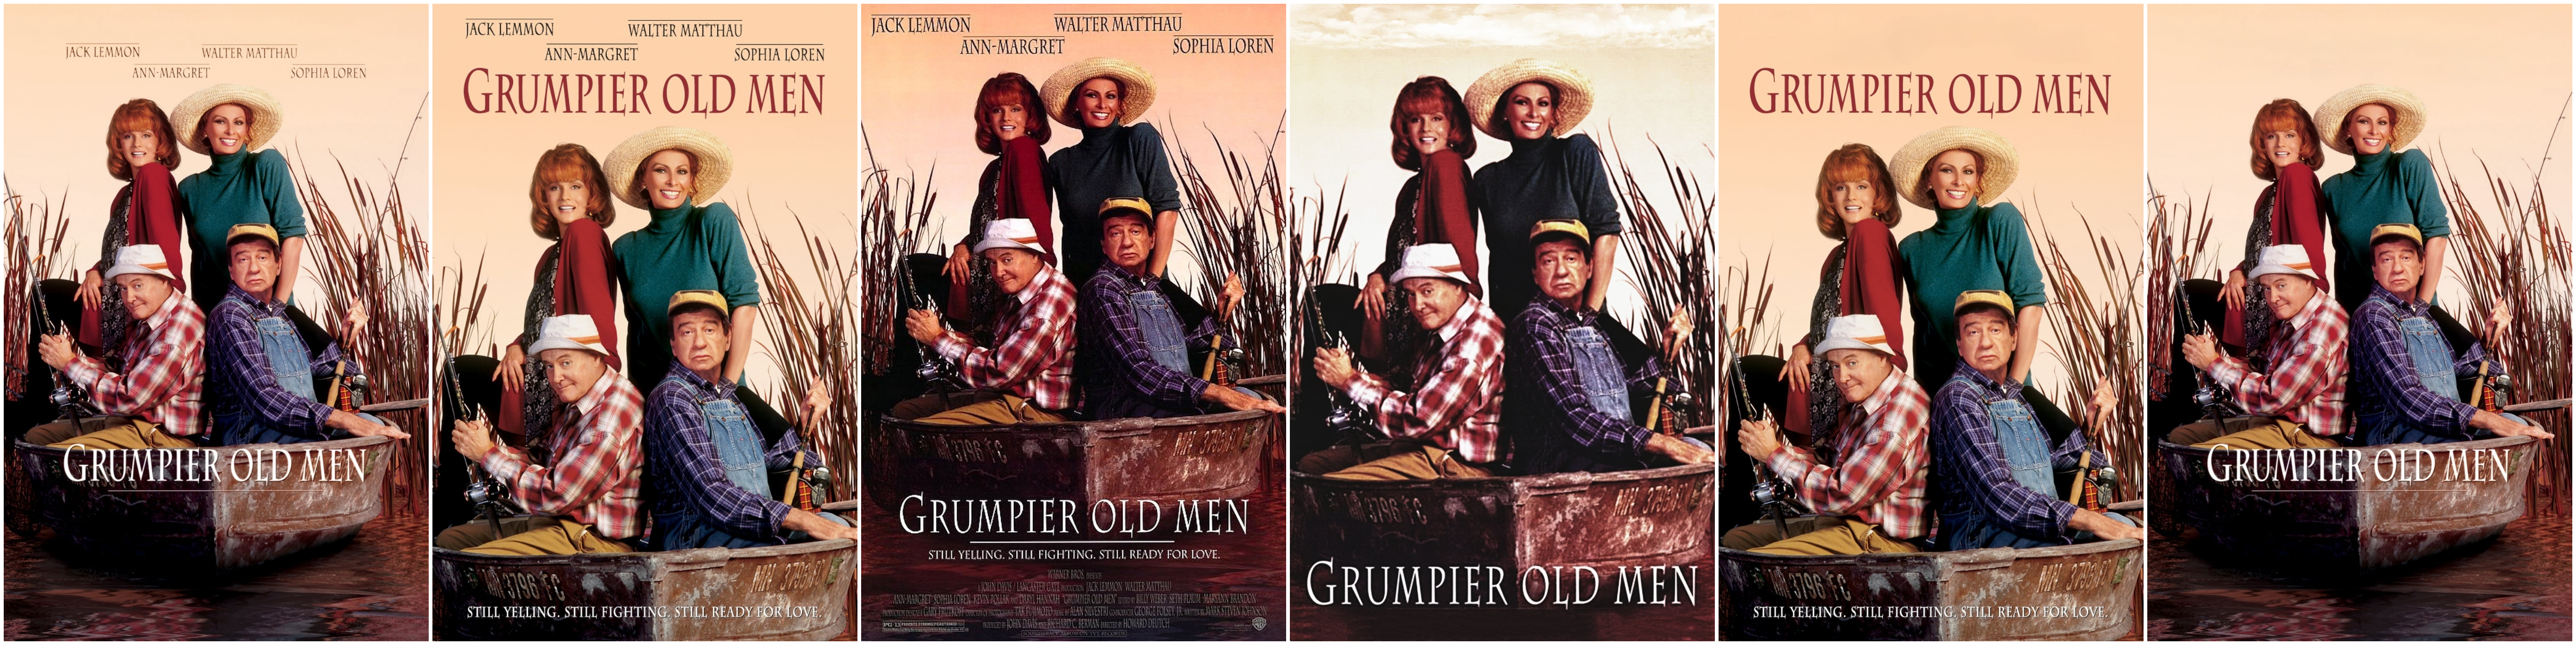
\includegraphics[width=\textwidth]{img_4_9}
  \end{subfigure}
  \hfill
  \begin{subfigure}[b]{0.48\textwidth}
    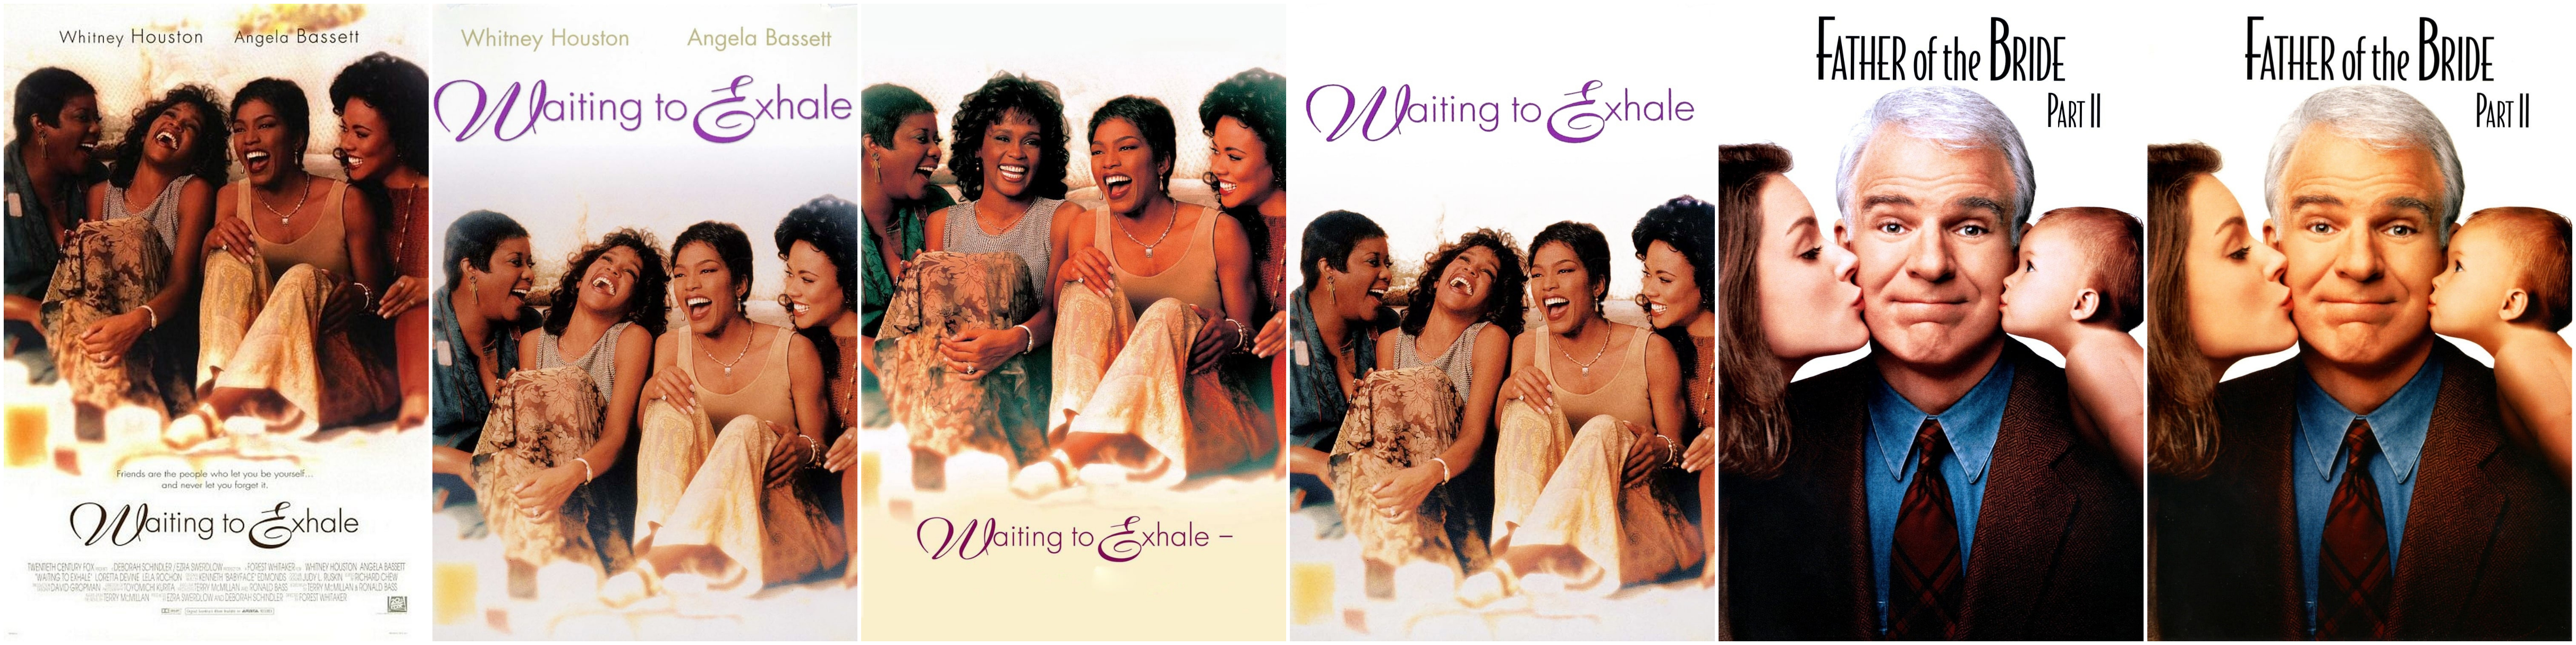
\includegraphics[width=\textwidth]{img_4_10}
  \end{subfigure}
  \hfill
  \begin{subfigure}[b]{0.48\textwidth}
    \includegraphics[width=\textwidth]{img_4_11}
  \end{subfigure}
  \hfill
  \begin{subfigure}[b]{0.48\textwidth}
    \includegraphics[width=\textwidth]{img_4_12}
  \end{subfigure}
    \hfill
  \begin{subfigure}[b]{0.48\textwidth}
    \includegraphics[width=\textwidth]{img_4_13}
  \end{subfigure}
    \hfill
  \begin{subfigure}[b]{0.48\textwidth}
    \includegraphics[width=\textwidth]{img_4_14}
  \end{subfigure}
      \hfill
  \begin{subfigure}[b]{0.3\textwidth}
    \includegraphics[width=\textwidth]{img_4_15}
  \end{subfigure}
  \caption[Postere input sanity check]{Posterele de input pentru sanity check.}
\end{figure}

Din punct de vedere al metricii de evaluare silhouette rezultatele se prezintă după cum urmează în figura 4.3.
\begin{figure}[!h]
	\centering
	\includegraphics[max width=12cm,max height=12cm,keepaspectratio]{img_4_16}
	\caption[Silhouette score pentru clasterele din sanity check]{Silhouette score pentru clasterele din sanity check.}
\end{figure} 

\subsection{Rezultate generale}

\section{Rezultate sistem de recomandare}
